\documentclass[UTF8,a4paper,12pt,fontset=none]{ctexart}

\usepackage[a4paper,margin=2.2cm]{geometry}
\usepackage{array}
\usepackage{booktabs}
\usepackage{caption}
\usepackage{enumitem}
\usepackage{float}
\usepackage{fontspec}
\usepackage{graphicx}
\usepackage{hyperref}
\usepackage{listings}
\usepackage{siunitx}
\usepackage{subcaption}
\usepackage{tabularx}
\usepackage{xurl}
\usepackage{xcolor}

\hypersetup{colorlinks=true,linkcolor=blue!60!black,urlcolor=blue!60!black}
\defaultCJKfontfeatures{AutoFakeSlant=.2}
\setCJKmainfont{Songti SC}
\setCJKsansfont{Heiti SC}
\setCJKmonofont{Heiti SC}
\setmonofont{Menlo}
\setlength{\parindent}{2em}
\setlength{\parskip}{0.35em}
\emergencystretch=3em
\graphicspath{{results/figures/}{../results/figures/}}
\captionsetup{font=small}
\sisetup{round-mode=places,round-precision=3}
\renewcommand{\figurename}{图}
\renewcommand{\tablename}{表}

\definecolor{CodeBg}{HTML}{F7F7F7}
\definecolor{CodeKeyword}{HTML}{1D4E89}
\definecolor{CodeComment}{HTML}{0B6E4F}
\definecolor{CodeString}{HTML}{C73E1D}

\lstset{
  basicstyle=\ttfamily\small,
  backgroundcolor=\color{CodeBg},
  frame=single,
  framerule=0pt,
  xleftmargin=1em,
  xrightmargin=1em,
  breaklines=true,
  columns=fullflexible,
  keywordstyle=\color{CodeKeyword}\bfseries,
  commentstyle=\color{CodeComment},
  stringstyle=\color{CodeString},
  showstringspaces=false
}

\title{\bfseries 中山大学计算机学院本科生实验报告}
\author{}
\date{}

\begin{document}

\begin{titlepage}
  \centering
  {\zihao{2}\bfseries 中山大学计算机学院本科生实验报告\par}
  \vspace{0.5em}
  {\zihao{4}（2025学年春季学期）\par}
  \vspace{2em}

  \begin{tabularx}{0.9\textwidth}{>{\bfseries}p{4cm}X}
    课程名称： & 并行程序设计与算法 \\
    实验题目： & Lab6 Pthreads 并行构造与 Heated Plate 并行应用 \\
    批改人： & \\
    专业（方向）： & \\
    学号： & 23336128 \\
    姓名： & 梁力航 \\
    Email： & \\
    完成日期： & 2026年5月7日 \\
  \end{tabularx}

  \vfill
  \begin{minipage}{0.88\textwidth}
    \small
    本次实验从课程给出的 \texttt{heated\_plate\_openmp.c} 出发，保留原来的边界条件
    和 Jacobi 迭代公式，只把内部网格的行循环换成自己写的 Pthreads
    \texttt{parallel\_for}。为了观察任务划分方式的影响，我另外做了
    \texttt{block}、\texttt{cyclic}、\texttt{dynamic} 三种调度，并把结果和 OpenMP
    版本放在同一套脚本里比较。
  \end{minipage}
\end{titlepage}

\section{实验目的}

Heated Plate 本身的计算并不复杂，难点在于每一轮迭代都有固定的数据依赖：新矩阵
只能从上一轮矩阵计算，不能直接原地更新。因此，本实验主要关注两件事：第一，怎样把
内部网格点的更新拆成可并行的循环；第二，手写的 Pthreads \texttt{parallel\_for}
和 OpenMP 版本相比，正确性和运行时间会有什么差别。

具体实验内容如下：
\begin{enumerate}[leftmargin=2.2em]
  \item 理解 Heated Plate 稳态热传导问题的迭代过程；
  \item 用 Pthreads 实现 \texttt{parallel\_for}，并接入 Heated Plate；
  \item 比较 \texttt{block}、\texttt{cyclic}、\texttt{dynamic} 三种调度方式；
  \item 与课程资料中的 OpenMP 实现做正确性和运行时间对照；
  \item 整理出可以复现实验的脚本、结果和报告。
\end{enumerate}

\section{实验平台与参考来源}

\begin{table}[H]
  \centering
  \caption{实验环境信息}
  \renewcommand{\arraystretch}{1.2}
  \begin{tabularx}{0.92\textwidth}{>{\bfseries}p{4cm}X}
    \toprule
    项目 & 配置 \\
    \midrule
    宿主机 & macOS / arm64 \\
    运行环境 & Docker Linux (Ubuntu 24.04, arm64) \\
    C++ 编译器 & \texttt{g++}，\texttt{-O3 -std=c++17 -pthread -fopenmp} \\
    并行模型 & OpenMP / Pthreads \\
    Python 工作流 & \texttt{uv run python ...} \\
    程序输出 & \texttt{key=value} 形式，便于脚本解析 \\
    \bottomrule
  \end{tabularx}
\end{table}

实验中用到的线程接口主要来自 POSIX Pthreads；计时部分 OpenMP 对照程序使用
\texttt{omp\_get\_wtime()}。相关接口参考如下：
\begin{itemize}[leftmargin=2.2em]
  \item Pthreads 线程创建和等待参考 POSIX \texttt{pthread\_create} / \texttt{pthread\_join}：
  \url{https://pubs.opengroup.org/onlinepubs/9699919799/functions/pthread_create.html}，
  \url{https://pubs.opengroup.org/onlinepubs/9699919799/functions/pthread_join.html}。
  \item Pthreads 动态调度中的共享游标使用互斥锁保护，参考 POSIX \texttt{pthread\_mutex\_lock}：
  \url{https://pubs.opengroup.org/onlinepubs/9699919799/functions/pthread_mutex_lock.html}。
  \item OpenMP 对照程序用 \texttt{omp\_get\_wtime()} 统计 wall-clock 时间，参考 OpenMP 5.0 文档：
  \url{https://www.openmp.org/spec-html/5.0/openmpsu160.html}。
\end{itemize}

\section{问题描述与并行化思路}

Heated Plate 使用二维规则网格描述矩形区域的温度。边界条件为：上边界温度为 0，左、
右和下边界温度为 100。内部点每轮迭代按照四邻域平均值更新：
\[
W_{i,j}^{new} = \frac{1}{4}(U_{i-1,j}+U_{i+1,j}+U_{i,j-1}+U_{i,j+1})
\]
当相邻两轮之间的最大变化量 \texttt{diff} 小于给定阈值 \texttt{epsilon} 时停止。

我采用的是 Jacobi 更新方式。每轮先把当前矩阵 \texttt{W} 复制到 \texttt{U}，再根据
\texttt{U} 算出新的 \texttt{W}。这样做虽然多了一次复制，但好处是同一轮里每个内部点
只读旧矩阵，写入的位置也互不重叠。因此可以把内部行交给不同线程处理，不需要在更新
矩阵时加锁。

\section{核心实现}

\subsection{\texttt{parallel\_for} 调度方式}

在 Lab5 的连续块划分基础上，我这里保留并扩展了三种调度：
\begin{itemize}[leftmargin=2.2em]
  \item \texttt{block}：将迭代空间按连续块均分给各线程；
  \item \texttt{cyclic}：每个线程按固定步长轮转领取 chunk；
  \item \texttt{dynamic}：多个线程通过互斥锁保护的共享游标动态领取 chunk。
\end{itemize}

其中 \texttt{dynamic} 的主要代码如下。它的思路是用一个共享游标记录下一个还没分配的
chunk，每个线程取任务时先加锁，取完后马上释放锁：
\begin{lstlisting}[language=C++]
pthread_mutex_lock(&shared->mutex);
iter_begin = shared->next_iter;
shared->next_iter += shared->chunk_size;
pthread_mutex_unlock(&shared->mutex);

if (iter_begin >= shared->total_iters) {
    break;
}
iter_end = std::min(iter_begin + shared->chunk_size, shared->total_iters);
execute_range(shared, iter_begin, iter_end);
\end{lstlisting}

\subsection{Heated Plate 并行化}

Pthreads 版本每一轮迭代拆成三个并行循环：
\begin{enumerate}[leftmargin=2.2em]
  \item 复制矩阵：\texttt{W -> U}；
  \item 更新内部行：根据 \texttt{U} 计算新的 \texttt{W}；
  \item 计算每一行的局部最大变化量，并由主线程规约得到全局 \texttt{diff}。
\end{enumerate}

计算 \texttt{diff} 时，我没有让多个线程直接更新同一个全局变量，而是先把每一行的局部
最大变化量写到 \texttt{row\_diff[i]}，最后由主线程顺序扫描。这种写法比较朴素，但结果
更容易检查，三种 Pthreads 调度和 OpenMP 对照也能得到相同的 checksum。

\section{实验结果}

我在仓库中保留了一组中等规模的测试结果，配置如下：
\begin{itemize}[leftmargin=2.2em]
  \item 网格规模：\(64\times64\)、\(128\times128\)、\(256\times256\)；
  \item 线程数：1、2、4；
  \item 阈值：\texttt{epsilon=0.1}；
  \item Pthreads chunk 大小：8；
  \item 每组运行次数：1。
\end{itemize}

完整数据保存在 \texttt{results/benchmark\_results.json}、
\texttt{results/summary\_by\_version.csv} 和 \texttt{results/performance\_table.csv}。
这组数据一共 36 条记录，状态均为 \texttt{ok}；Pthreads 三种调度方式和 OpenMP 对照
的 checksum 也保持一致。

\begin{table}[H]
  \centering
  \caption{部分运行时间结果（秒）}
  \renewcommand{\arraystretch}{1.15}
  \begin{tabular}{llrrr}
    \toprule
    后端 & 版本 / 调度 & 线程数 & \(128\times128\) & \(256\times256\) \\
    \midrule
    OpenMP & \texttt{openmp\_original} & 1 & 0.012308 & 0.019530 \\
    OpenMP & \texttt{openmp\_original} & 2 & 0.001909 & 0.008796 \\
    Pthreads & \texttt{block} & 1 & 0.028204 & 0.045497 \\
    Pthreads & \texttt{block} & 2 & 0.024976 & 0.029151 \\
    Pthreads & \texttt{cyclic} & 2 & 0.030628 & 0.031942 \\
    Pthreads & \texttt{dynamic} & 2 & 0.033584 & 0.055894 \\
    \bottomrule
  \end{tabular}
\end{table}

\begin{figure}[H]
  \centering
  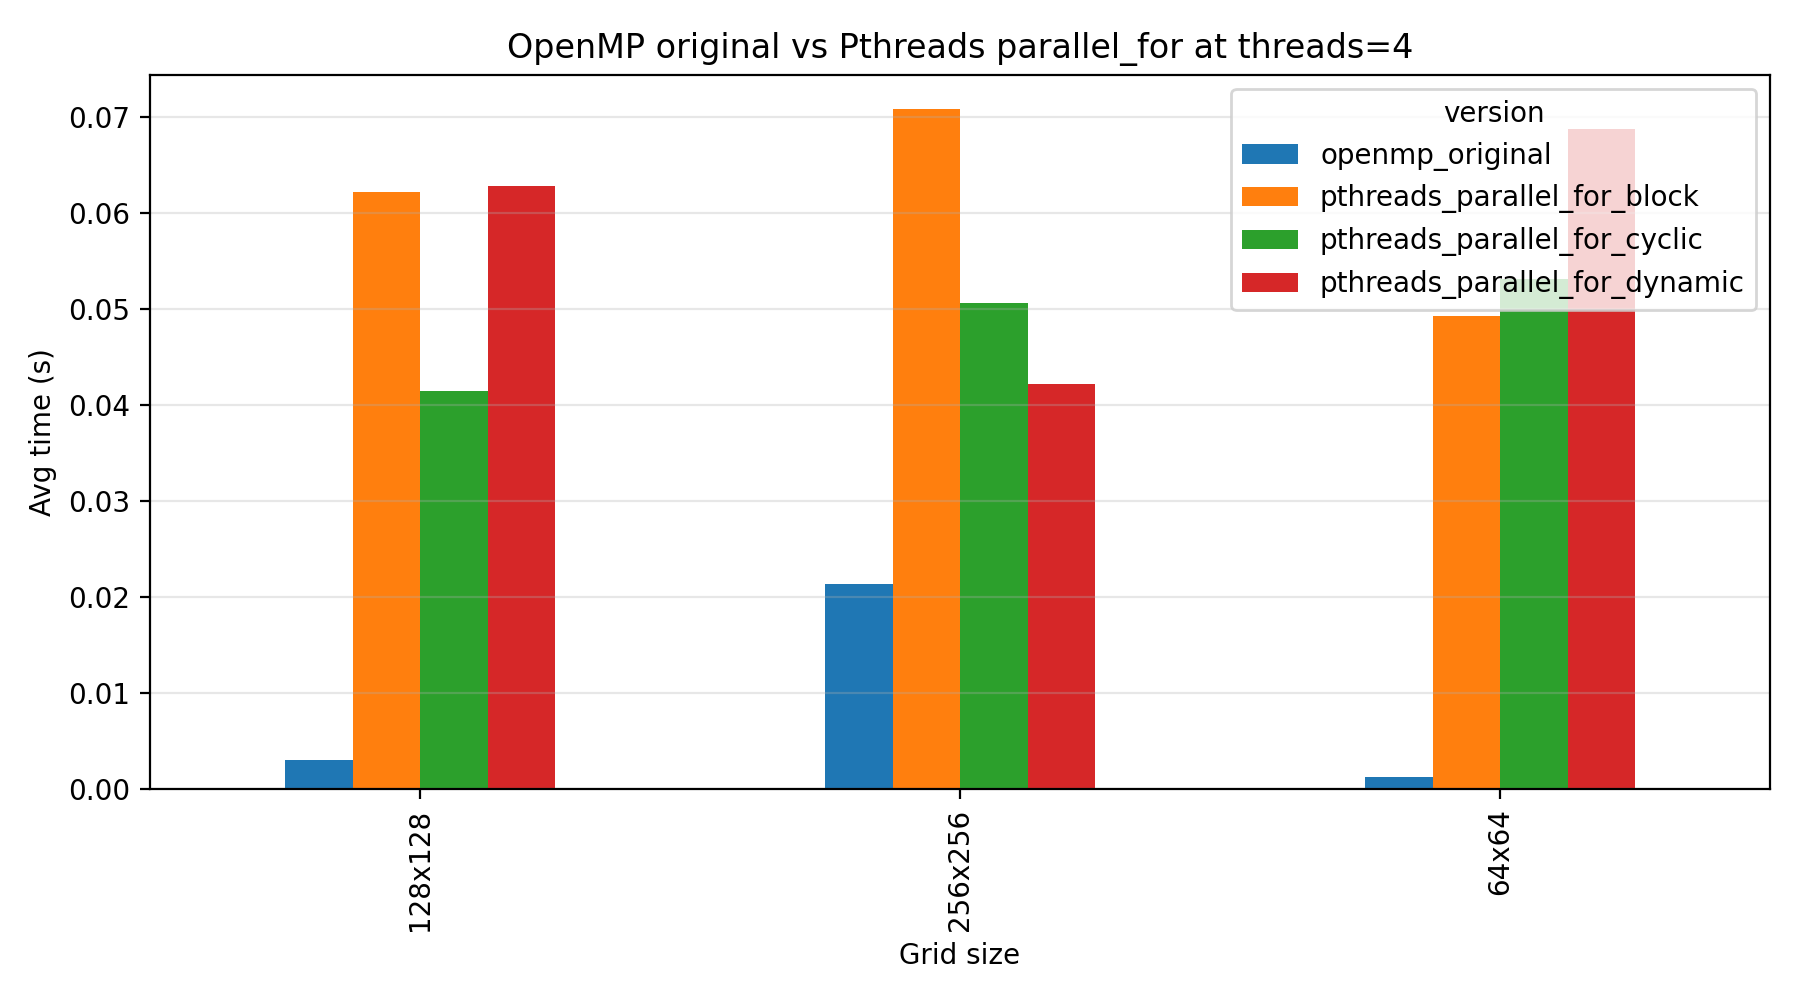
\includegraphics[width=0.82\textwidth]{openmp_vs_pthreads.png}
  \caption{OpenMP 原始实现与 Pthreads \texttt{parallel\_for} 版本对比}
\end{figure}

\begin{figure}[H]
  \centering
  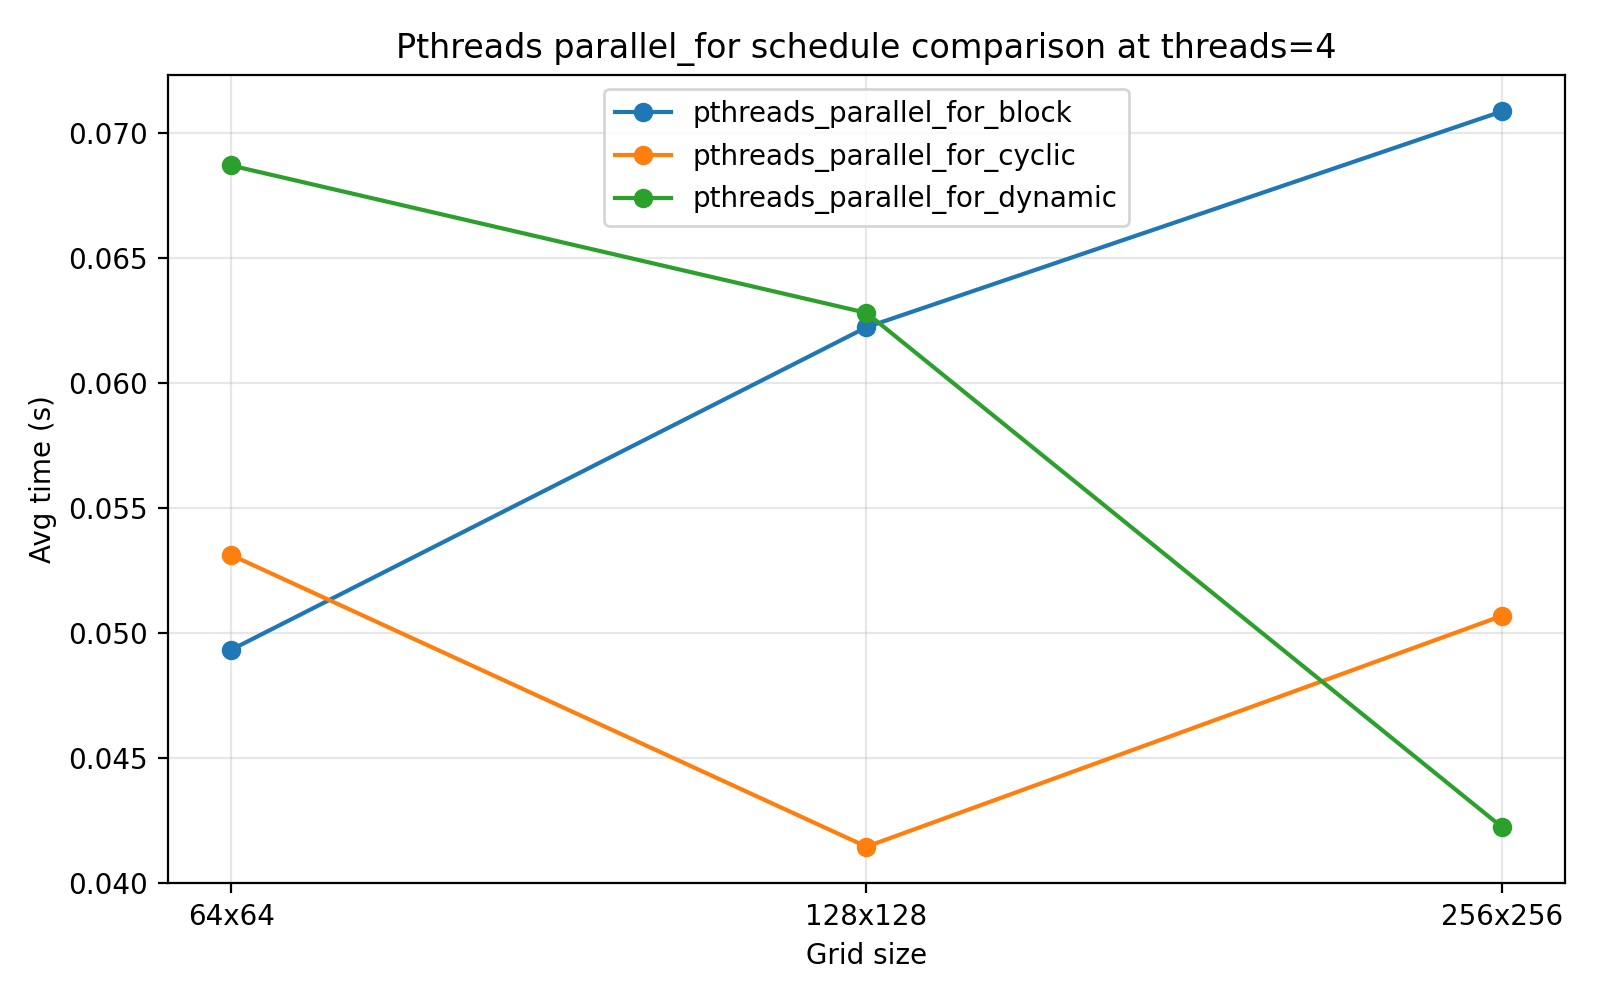
\includegraphics[width=0.82\textwidth]{pthreads_schedule_comparison.png}
  \caption{Pthreads \texttt{parallel\_for} 三种调度方式对比}
\end{figure}

\begin{figure}[H]
  \centering
  \begin{subfigure}{0.48\textwidth}
    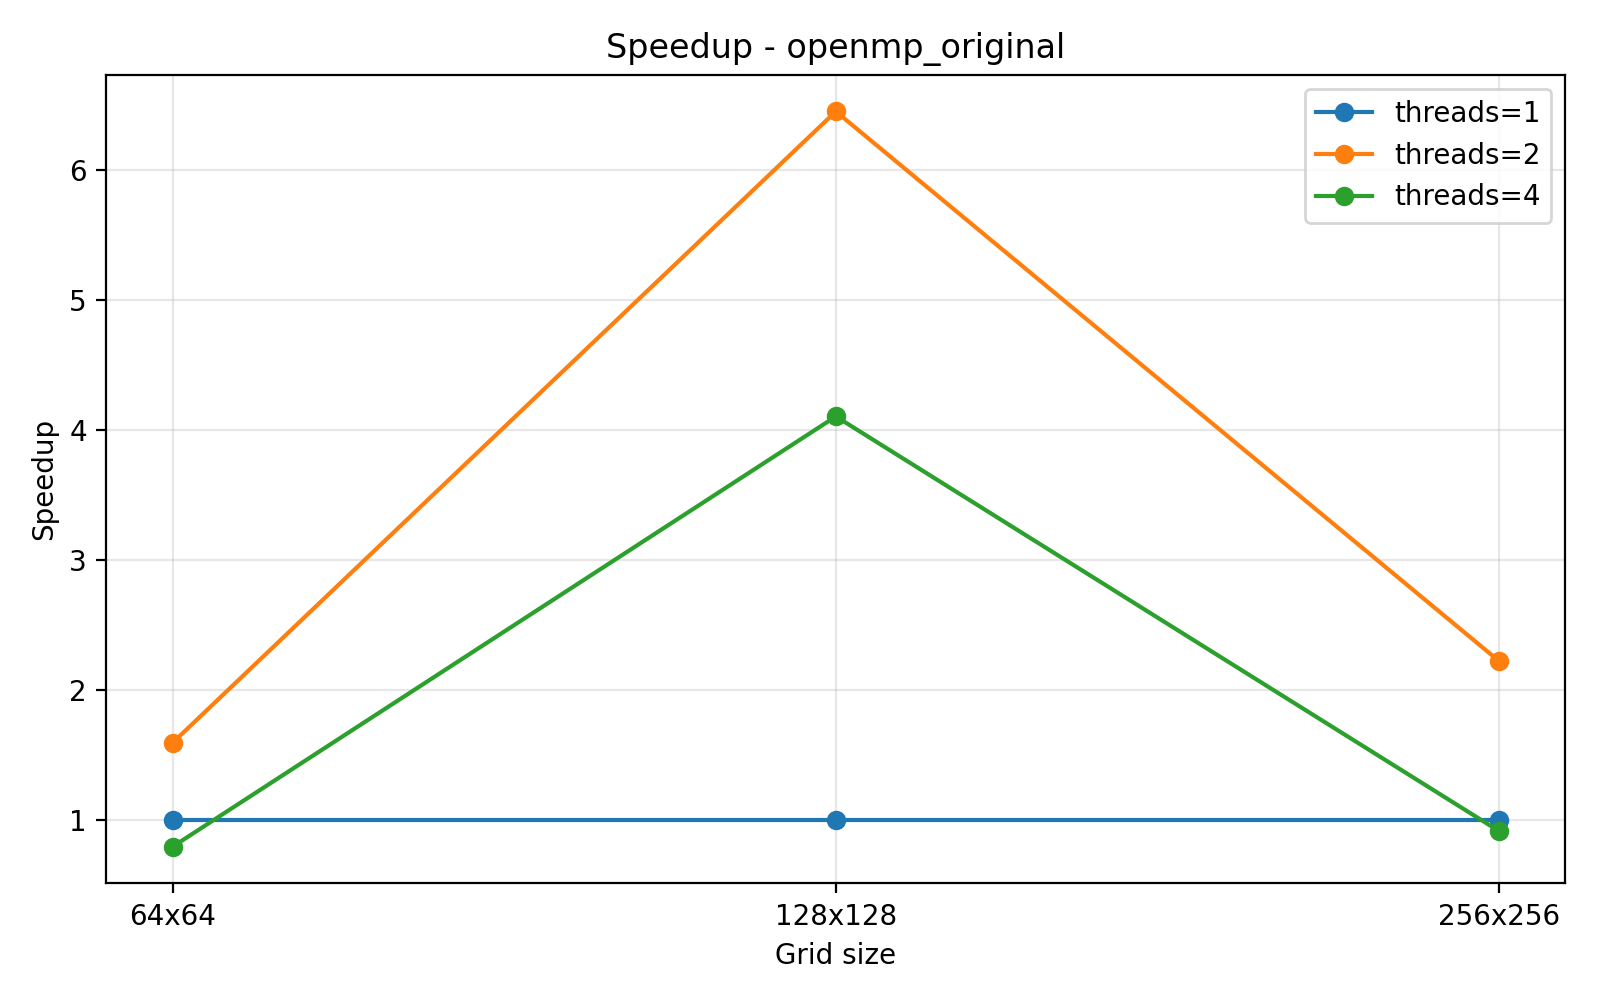
\includegraphics[width=\textwidth]{speedup_openmp_original.png}
    \caption{OpenMP speedup}
  \end{subfigure}
  \hfill
  \begin{subfigure}{0.48\textwidth}
    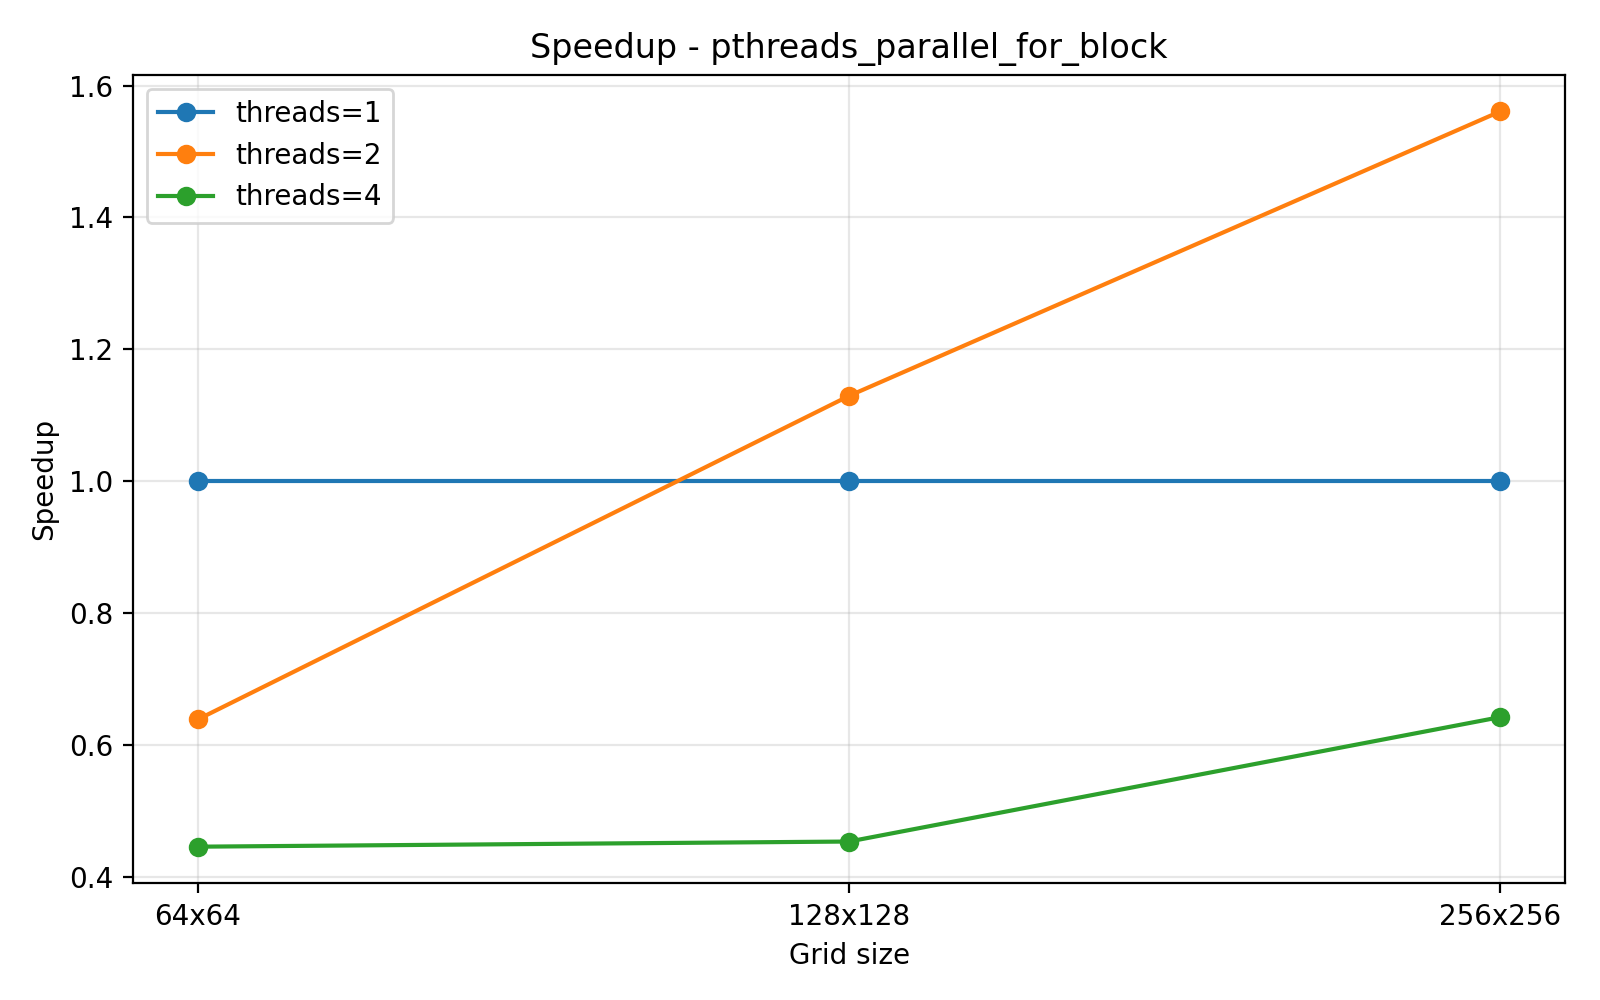
\includegraphics[width=\textwidth]{speedup_pthreads_parallel_for_block.png}
    \caption{Pthreads block speedup}
  \end{subfigure}
  \caption{加速比曲线示例}
\end{figure}

\section{结果分析}

从表格和图中可以看到，OpenMP 版本整体明显更快。这个结果并不意外。两边的数值计算公式
是一样的，差距主要来自运行时开销：我写的 \texttt{parallel\_for} 每调用一次都会创建一批
Pthreads 线程，执行完再回收；而 Heated Plate 每轮迭代里至少要并行执行复制、更新和
计算 \texttt{diff} 三段循环，线程管理开销被重复放大了。

三种 Pthreads 调度之间，\texttt{block} 在这个问题上反而更稳。原因是规则网格里每一行
的计算量基本相同，连续分块已经能把任务分得比较均匀。\texttt{dynamic} 的优势一般出现在
任务不均衡时，但这里每次取 chunk 都要访问互斥锁，额外开销抵消了它的灵活性。
\texttt{cyclic} 可以把行号打散，但对本实验这种规则访问模式来说，没有明显收益。

\section{验证}

为了避免只看运行时间而忽略正确性，我写了两组测试：
\begin{itemize}[leftmargin=2.2em]
  \item \texttt{tests/test\_core\_programs.py}：验证 OpenMP 与三种 Pthreads 调度的
  checksum 和迭代次数一致，验证 \texttt{--dump} 输出和动态库链接；
  \item \texttt{tests/test\_benchmark.py}：用缩小配置跑通 benchmark、plot 和
  export 流程，检查 JSON、CSV、图表和表格产物。
\end{itemize}

本次提交前执行了：
\begin{lstlisting}[language=bash]
uv run python -m unittest ./tests/test_core_programs.py
uv run python -m unittest ./tests/test_benchmark.py
\end{lstlisting}

两组测试均通过。额外检查了 benchmark 结果文件，其中 36 条记录均为 \texttt{ok}。

\section{结论}

本次实验完成了 Heated Plate 从 OpenMP 参考程序到 Pthreads \texttt{parallel\_for} 版本的
改造。三种调度方式都能得到和 OpenMP 对照一致的迭代次数与 checksum，说明并行拆分没有破坏
Jacobi 迭代的计算逻辑。

性能方面，手写 \texttt{parallel\_for} 版本没有超过 OpenMP。这个结果也说明了一个问题：
仅仅把循环拆给多个线程并不等于一定更快，线程创建、同步和任务划分本身也会消耗时间。如果
继续优化，我会优先把 \texttt{parallel\_for} 改成持久线程池，让多个迭代阶段复用同一批线程，
而不是每次进入并行循环都重新创建线程。

\end{document}
